%%====================================================================
\documentclass[10pt,a4paper,twocolumn,showkeys,showpacs,aps,groupedaddress,noeprint]{revtex4-1}
%\documentclass[portuguese,10pt,twocolumn]{article}
%\documentclass[12pt,a4paper,oneside,twocolumn]{book}
%====================================================================
\usepackage[english,portuguese,brazilian,brazil]{babel}
\usepackage[text={17cm,25.0cm},centering]{geometry}
%\usepackage[latin1]{inputenc}  % Antiga codificação padrão
\usepackage[utf8]{inputenc}     % Atualmente é a codificação padrão
%\usepackage{indentfirst}       % indenta os primeiros parágrafos
\usepackage{amsmath,amssymb,amsfonts}
\usepackage{amsthm}
%\usepackage{theorem}
%\usepackage[num]{abntcite}
%\usepackage[alf]{abntcite}
%\usepackage{cite}
%  Tabelas
%\usepackage{bm}       % Letras gregas negrito
\usepackage{textcomp} % simbolos especiais
%\usepackage{supertabular}
%\usepackage{multirow}
\usepackage{xcolor}
%\usepackage{booktabs}
\usepackage{colortbl}
%\usepackage{xtab}
%\usepackage{hhline}
\usepackage{comment} % ambiente comentário \begin{comment}
\usepackage{lipsum}% for dummy text


%\usepackage[pdfborder={0 0 0},colorlinks,linkcolor=black,anchorcolor=black,citecolor=black]{hyperref}
\usepackage{hyperref}
%---------------------------------------------------------------------
\hypersetup{
   pdfborder={0 0 0},            % Sem caixa em volta da hiperreferência
   pdftoolbar=true,              % Mostra a barra de ferramentas no Acrobat Reader = true ==> sim
   pdfmenubar=true,              % Mostra o menu no Acrobat Reader = true ==> sim
   pdffitwindow=false,           % Ajusta o documento ao tamanho da janela aberta = false==> não
   pdfstartview={FitH},          % Ajusta a largura da página a da janela aberta 
   pdfauthor={Salviano A. Leão}, % Autor do documento
   pdftitle={Modelo de artigo},  % Titulo do documento
   pdfsubject={Modelo},          % Assunto do documento
   pdfkeywords={Modelo,artigo},  % Palavras chaves do documento
   pdfproducer={LaTeX},    % O produtor do documento
   pdfcreator={pdfLaTeX},  % O programa que criou o documento
   pdfnewwindow=true,      % Abre links em uma nova janela
   colorlinks=true,       % false: links em uma caixa; true: links coloridos
   linkcolor=red,          % Cor dos links internos (mude a cor da caixa com linkbordercolor)
   citecolor=green,        % Cor dos links das referências bibliográficas
   filecolor=magenta,      % Cor dos links dos arquivos
   urlcolor=cyan           % Cor dos links externos
}
%Note que o último item não tem vírgula.
%--------------------------------------------------------------------
\usepackage{graphicx} 
%====================================================================
\DeclareGraphicsExtensions{.eps,.png,.jpg,.pdf}
%\DeclareGraphicsRule{.eps}{eps}{.bb}{`jpeg2ps -h -r 1200 #1}
%\DeclareGraphicsRule{.eps}{eps}{.bb}{`jpeg2ps -h -r 600 #1}
%\DeclareGraphicsRule{.eps}{eps}{.bb}{`jpeg2ps -h -r 300 #1}
%\DeclareGraphicsRule{.eps}{eps}{.bb}{`jpeg2ps -h -r 150 #1}
%\DeclareGraphicsRule{.eps}{eps}{.bb}{`jpeg2ps -h -r 100 #1}
%====================================================================
% Você pode deixar todas as suas figuras num único diretório e dizer
% aqui em qual diretório elas estão localizadas.
\graphicspath{
{Figs/} %%Local em que o latex ira buscar as figuras
%{/home/salviano/Cursos/Figs_Ensino/Aurora_Borealis/}
% {/home/salviano/Cursos/Figs_Ensino/Eletricidade/}
% {/home/salviano/Cursos/Figs_Ensino/}
%{/home/salviano/Cursos/Figs_Ensino/Eletricidade/}
% {/home/salviano/Cursos/Figs_Ensino/Eletricidade/Imagens_jpg/}
% {/home/salviano/Figuras/IF/}
% {coloque aqui onde estarao suas figuras}
}
%====================================================================
\usepackage{fancyhdr}
%\usepackage{makeidx}
\usepackage{float}
\usepackage{subfig}
%\usepackage{wrapfig}
% Para descentralizar o caption use os seguintes pacotes
\usepackage{caption}
%\usepackage{subcaption}
\usepackage{ragged2e}
\DeclareCaptionJustification{justified}{\justifying}
\captionsetup{justification=justified,singlelinecheck=false,labelfont=small,textfont={small,it}}
%labelfont=it,textfont={bf,it}
%====================================================================
% \newtheorem{theorem}{Teorema}
% \newtheorem{acknowledgement}[theorem]{Agradecimentos}
% \newtheorem{algorithm}[theorem]{Algoritmo}
% \newtheorem{axiom}[theorem]{Axioma}
% \newtheorem{case}[theorem]{Caso}
% \newtheorem{claim}[theorem]{Declaração}
% \newtheorem{conclusion}[theorem]{Conclução}
% \newtheorem{condition}[theorem]{Condição}
% \newtheorem{conjecture}[theorem]{Conjectura}
% \newtheorem{corollary}[theorem]{Corolário}
% \newtheorem{criterion}[theorem]{Critério}
% \newtheorem{definition}[theorem]{Definição}
\newtheorem{postulado}{Postulado}
% \newtheorem{example}{Exemplo}
% \newtheorem{exercise}{Exercício}
% \newtheorem{lemma}[theorem]{Lema}
% \newtheorem{notation}[theorem]{Notação}
% \newtheorem{problem}{Problema}
% \newtheorem{proposition}[theorem]{Proposição}
% \newtheorem{remark}[theorem]{Nota}
% \newtheorem{solution}{Solução}
% \newtheorem{summary}[theorem]{Sumário}
% \newenvironment{proof}[1][Prova]{\textbf{#1.} }{\ \rule{0.5em}{0.5em}}
%%====================================================================
\def\limfunc#1{\mathop{\rm #1}}
\def\func#1{\mathop{\rm #1}\nolimits}
\def\unit#1{\mathop{\rm #1}\nolimits}
%%====================================================================
% \setlength{\textwidth}{17.0cm}
% \setlength{\textheight}{24.5cm}
% \setlength{\parindent}{1.5cm}
% \setlength{\baselineskip}{0.8cm}
% \hoffset=-2.50cm
% \voffset=-2.0cm
%%====================================================================
% \renewcommand{\baselinestretch}{1.25}
% \renewcommand{\textfraction}{0.03}
% \renewcommand{\topfraction}{0.97}
% \renewcommand{\bottomfraction}{0.97}
%%====================================================================
% \thispagestyle{plain}
% \pagestyle{fancy}
% %\setlength{\headrulewidth}{0.6pt}
% \renewcommand{\headrulewidth}{0.6pt}
% \addtolength{\headwidth}{\marginparsep}
% \lhead[\fancyplain{}{\bfseries Salviano A. Leão}]%
%       {\fancyplain{}{\bfseries Salviano A. Leão}}
% \rhead[\fancyplain{}{\bfseries\leftmark}]%
%       {\fancyplain{}{\bfseries\thepage}}
% \cfoot{}

%%====================================================================
\hyphenation{a-tu-al}
\hyphenation{Fe-de-ral fe-de-ral}
\hyphenation{he-te-ro-es-tru-tu-ra he-te-ro-es-tru-tu-ras}
\hyphenation{es-pa-lha-do es-pa-lha-dos }
\hyphenation{co-ti-di-ano}
\hyphenation{ele-tri-ci-da-de}
\hyphenation{ex-pe-ri-men-tal}
\hyphenation{nu-cle-ar nu-cle-ares}
\hyphenation{ele-tri-ca-men-te}
\hyphenation{es-ta-be-le-cen-do}
%%====================================================================
%\input{Sal_Def}
%\input{tcilatex}
%%====================================================================
%-------------------------------------------------------------------------------
\definecolor{gold}{rgb}{0.85,.66, 0}
\definecolor{azul_escuro}{rgb}{0.12,0.26, 0.36}
\definecolor{azul}{rgb}{0.21,0.55, 0.0}
\definecolor{Azul}{rgb}{0.21,0.85,0.85}
\definecolor{laranja}{rgb}{0.95,.65, 0.20}
\definecolor{amarelo}{rgb}{0.95,.95, 0.55}
\definecolor{amarelo1}{rgb}{1,0.97, 0.20}
\definecolor{amarelo2}{rgb}{0.85,0.55, 0.0}
\definecolor{amarelo3}{rgb}{1.0,1.0, 0.80}
\definecolor{Amarelo}{rgb}{0.99,0.99, 0.66}
\definecolor{verde}{rgb}{0.57,0.94, 0.80}
\definecolor{Cinza50}{gray}{0.50}
\definecolor{Cinza10}{gray}{0.10}
\definecolor{Cinza}{gray}{0.80}
\definecolor{cinza}{rgb}{0.9,0.9,0.9}
%-----------------------------------------------------------------------------------
%Definições de tabelas

%-------------------------------------------------------------------------------
\newlength{\LC}
\setlength{\LC}{7.0cm}
\newcolumntype{A}{>{\columncolor[gray]{0.96}\raggedright\color{blue}}l}
\newcolumntype{B}{>{\columncolor[gray]{0.96}\raggedright\color{blue}}r}
\newcolumntype{F}{>{\columncolor[gray]{0.95}\raggedright}m{\LC}}
\newcolumntype{G}{>{\columncolor[gray]{0.9}\raggedright}m{1.70cm}}
\newcolumntype{K}{>{\columncolor[gray]{0.8}\raggedright}c}
\newcolumntype{H}{>{\columncolor{yellow}\raggedright}c}
%-------------------------------------------------------------------------------

\begin{document}

\title{Aqui o título do paper}
\author{Salviano de A. Leão}\email{salviano@ufg.br}
\affiliation{Instituto de Física,\\
Universidade Federal de Goiás,\\
C.P.131, 74.001-970,\\
Goiânia (GO), Brasil}
\author{João Ninguém}\email{joao.niquem@gmail.com}
\affiliation{Instituto de Física de Lugar Nenhum,\\
Universidade Federal de Lugar Nenhum,\\
C.P.777, 99.999-999,\\
Lugar Nenhum (XX), Brasil}
%\date{Novembro de 2009}

\begin{abstract}
   Aqui deve vir o resumo do seu trabalho. Você deve explicar
   de forma sucinta o que você fez
\end{abstract}

\keywords{Palavra-chave01, Palavra-chave02, Palavra-chave03}

\maketitle

\section{Elementos de um Circuito}

\lipsum[1]

O livro de eletromagnetismo ideal é o do Griffiths 
\cite{GriffithsEletro}, o qual porém o 
do \cite[ver pag.10]{Adams1992,Niguem2013}.

Para analisarmos\cite{Campos2001,Heath1997,Dahlquist1974} um circuito 
precisamos conhecer os elementos que compõem o
mesmo. Vamos fazer um teste para citar \cite{Tort2001,Adams1992}.

Será feita uma simulação numérica\cite{Conte1980} dos resultados, e
para tal \ldots

\begin{equation}\label{eq:Sch} 
   i \hbar \dfrac{\partial \psi}{\partial t} = H \psi
\end{equation} 

\begin{postulado}
   Enuncia-se o postulado 1. \lipsum[2]
\end{postulado}


\subsection{Resistor}

Um \href{https://www.google.com.br}{resistor} (ôhmico, ou seja, aquele que obedece a lei de Ohm, $V=RI$)
é um elemento de circuito, representado pelo símbolo da figura 
\ref{fig:Resistor}. A lei de Ohm nos diz que: Quando por um resistor R passar
uma corrente I, haverá uma queda de potencial (no sentido da corrente:
$V=V_{1}-V_{2}$; $V_{1}>V_{2}$), através dos seus extremos 1 e 2, dada
por:
\begin{equation*}
V=RI
\end{equation*}

\begin{figure}[!h]
\begin{center}
\includegraphics[width=0.70\linewidth]{Resistor_02.eps}
\end{center}
\caption[]{A figura mostra um elemento de circuito denominado por resistor. O 
resistor possui uma resistência de 20,0 $\Omega$.}
\label{fig:Resistor}
\end{figure}


Num resistor, há uma conversão de energia elétrica em energia
térmica, dada pelo efeito Joule. A potência dissipada pelo resistor
devido ao efeito Joule é dada por\cite{RLandau97,DeVries93}:
\begin{equation*}
P=RI^{2}=VI
\end{equation*}
\lipsum[3]
\begin{equation}
M =
\begin{pmatrix}
1/a & x & x \\
-\cos\gamma/(a\sin\chi) & 2 & x \\
x & x & 3
\end{pmatrix}
\end{equation}

Na superfície da figura

\begin{figure}[!h]
\begin{center}
\includegraphics[width=0.70\linewidth,angle=-90]{Superficie.eps}
\end{center}
\caption{Teste 2. \protect\lipsum[3]}
\label{Resistor}
\end{figure}

Este gráfico foi feito no gnuplot usando
o modo pm3d. Na equação de Scrodinger (\ref{eq:Sch})
ou \eqref{eq:Sch}

\begin{comment}
Alguns dos comandos fornecidos pelo Scilab para gerenciar as funções
são apresentadas na tabela~\ref{tab:GenFunc} abaixo.
\begin{table}[!htb]
\begin{center}
\begin{tabular}{ A| m{10.0cm}}
\hline
\rowcolor[gray]{.8}
\textbf{Função}    &
\textbf{Significado} \\
\hline
\texttt{function}    & abre a definição de uma função \\
\texttt{endfunction} & fecha a definição de uma função \\
\hline
\texttt{argn}      & número de argumentos de entrada/saída de uma função\\
\texttt{varargin}  & variável com o número de argumentos da lista de entrada\\
\texttt{varargout} & variável com o número de argumentos da lista de saída\\
\hline
\texttt{fun2string}          & gera a definição ASCII de uma função do Scilab\\
\texttt{get\_function\_path} & obtém o caminho do arquivo fonte de uma biblioteca de funções\\
\texttt{getd}                & obtém todas as funções definidas em um diretório\\
\texttt{head\_comments}      & mostra o cabeçalho de comentários das funções do Scilab\\
\texttt{listfunctions}       & lista as propriedades de todas as funções no ambiente do Scilab\\
\texttt{macrovar}            & variáveis de uma função\\
\hline
\end{tabular}
\end{center}
\caption{Funções do Scilab para gerenciar funções.}
\label{tab:GenFunc}
\end{table}
\end{comment}

%\setlength\arrayrulewidth{2pt}\arrayrulecolor{blue}
%\setlength\doublerulesep{2pt}\doublerulesepcolor{blue}
\begin{table}
\begin{center}
\begin{tabular}{c | c | c}
0 & 2 & 3\\ \hline
\rowcolor{cinza}\multicolumn{1}{c}{5} & \multicolumn{1}{c}{5} & \multicolumn{1}{c}{5} \\
\hline
\rowcolor[gray]{.8} 1 & 1 & 1\\
4 & 6 & 8
\end{tabular}
\end{center}
\end{table}


\section{Método numérico}

O Método das Diferenças Finitas (MDF) é um método geralmente
utilizado para resolver equações diferenciais. Inicialmente
discretizamos o espaço, e esta discretização poderá ser
uniforme ou não e posteriromente reescrevemos a equação\cite[ver pag. 34]{RLandau97}
diferencial em termos das diferenças. Nos casos que iremos estudar
agora, iremos considerar uma discretização não uniforme,
conforme a figura ~\ref{fig2} abaixo.

\begin{equation}
   x^2\Longleftrightarrow
\end{equation} 

\begin{figure}[htb]
\begin{center}
\setlength{\unitlength}{0.0040in}%
\begin{picture}(565,100)(15,450)
\thicklines
\put(150,480){\circle*{7}}
\put(170,480){\circle*{7}}
\put(190,480){\circle*{7}}
\put(415,480){\circle*{7}}
\put(435,480){\circle*{7}}
\put(455,480){\circle*{7}}
\put(-53,480){\line( 1, 0){185}}
\put(-60,480){\circle{15}}
%%\put(-60,490){\line( 0,-1){ 20}}
%%\put( 20,480){\line( 1, 0){100}}%%
%%\put( 20,490){\line( 0,-1){ 20}}
\put( 20,480){\circle*{15}}
\put( 20,470){\line( 0, 1){  0}}
%%\put(100,490){\line( 0,-1){ 20}}
\put(100,480){\circle*{15}}
\put(200,480){\line( 1, 0){200}}
\put(220,480){\circle*{15}}
\put(300,480){\circle*{15}}
\put(380,480){\circle*{15}}
\put(500,480){\circle*{15}}
\put(580,480){\circle*{15}}
%\put(220,490){\line( 0,-1){ 20}}
%\put(300,490){\line( 0,-1){ 20}}
%\put(380,490){\line( 0,-1){ 20}}
%\put(500,490){\line( 0,-1){ 20}}
%\put(580,490){\line( 0,-1){ 20}}
\put(480,480){\line( 1, 0){173}}
%\put(660,490){\line( 0,-1){ 20}}
\put(660,480){\circle{15}}
\put(225,500){\makebox(0,0)[lb]{\raisebox{0pt}[0pt][0pt]{ $\Delta x_{i-1}$}}}
\put(320,500){\makebox(0,0)[lb]{\raisebox{0pt}[0pt][0pt]{ $\Delta x_{i}$}}}
\put(-65,440){\makebox(0,0)[lb]{\raisebox{0pt}[0pt][0pt]{\large $0$}}}
\put( 15,440){\makebox(0,0)[lb]{\raisebox{0pt}[0pt][0pt]{\large $1$}}}
\put( 95,440){\makebox(0,0)[lb]{\raisebox{0pt}[0pt][0pt]{\large $2$}}}
\put(195,440){\makebox(0,0)[lb]{\raisebox{0pt}[0pt][0pt]{\large $i-1$}}}
\put(295,440){\makebox(0,0)[lb]{\raisebox{0pt}[0pt][0pt]{\large $i$}}}
\put(357,440){\makebox(0,0)[lb]{\raisebox{0pt}[0pt][0pt]{\large $i+1$}}}
\put(473,440){\makebox(0,0)[lb]{\raisebox{0pt}[0pt][0pt]{\large $n-1$}}}
\put(572,440){\makebox(0,0)[lb]{\raisebox{0pt}[0pt][0pt]{\large $n$}}}
\put(632,440){\makebox(0,0)[lb]{\raisebox{0pt}[0pt][0pt]{\large $n+1$}}}
%\put(247,490){\makebox(0,0)[lb]{\raisebox{0pt}[0pt][0pt]{\large $i-1$}}}
%\put(345,490){\makebox(0,0)[lb]{\raisebox{0pt}[0pt][0pt]{\large $i$}}}
\end{picture}
\end{center}
\vspace{-0.2cm}
\caption{Discretiza\c{c}\~{a}o da rede. \protect\lipsum[4] \label{fig2}}
\end{figure}%


Aqui iremos nos restringir a problemas em que temos equações
diferenciais de no máximo segunda ordem. Consideremos a expansão em 
série de Taylor da função $f(x)$ em torno do ponto $x_{i}$ (ver
figura ~\ref{fig2}). Na figura ~\ref{fig2} onde o índice $i$ indica um
ponto da rede discretizada, onde $f_{i}=f(x_{i})$ é o valor da 
função $f(x_{i})$ neste ponto e $\Delta _{i}=\Delta x_{i}=x_{i+1}-x_{i}$,
conforme mostra a figura~\ref{fig2}. Neste tipo de problema é muito
comum usarmos as seguintes condições de contorno: $f_{0}=f_{n+1}=0$,
$\Delta _{0}=\Delta _{1}$ e $\Delta _{n}=\Delta _{n-1}$.

\begin{align}
f(x+\Delta x_{i}) = & f(x) +\Delta x_{i}f^{\prime }(x) 
+\dfrac{\Delta x_{i}^{2}}{2!}f^{\prime \prime }(x) + \notag \\
& O(\Delta x_{i}^{3}) \label{df0}
\end{align}

\begin{align}
f(x+\Delta x_{i}) = & f(x)+\Delta x_{i}f^{\prime }(x)+
\dfrac{\Delta x_{i}^{2}}{2!}f^{\prime \prime }(x) + \notag \\ 
& O(\Delta x_{i}^{3})  \label{df1}
\end{align}

\begin{align}
f(x-\Delta x_{i-1}) = & f(x)-\Delta x_{i-1}f^{\prime }(x)+
\dfrac{\Delta x_{i-1}^{2}}{2!}f^{\prime \prime }(x) + \notag \\ 
& O(\Delta x_{i-1}^{3})  \label{df2}
\end{align}

\begin{align}
  & f(x+\Delta x_{i}) +f(x-\Delta x_{i-1}) \cong  2f(x) + \notag \\ 
  &\left( \Delta x_{i}-\Delta x_{i-1}\right) f^{\prime }(x) +
 \dfrac{(\Delta x_{i-1}^{2}+\Delta x_{i}^{2})}{2}f^{\prime \prime }(x)  
 \label{df3}
\end{align}

\begin{align}
  & f(x+\Delta x_{i}) - f(x-\Delta x_{i-1})  \cong  \notag \\ 
  & \left( \Delta x_{i-1} + \Delta x_{i} \right) f^{\prime }(x) -
 \dfrac{(\Delta x_{i-1}^{2}-\Delta x_{i}^{2})}{2} f^{\prime \prime }(x) \label{df4}
\end{align}
Podemos reescrever a eq. (\ref{df4}) como:

\begin{align}
f^{\prime }(x) & = \dfrac{f(x+\Delta x_{i})-f(x-\Delta x_{i-1})}{\Delta
x_{i-1}+\Delta x_{i}} - \notag \\ 
 & \dfrac{(\Delta x_{i}-\Delta x_{i-1})}{2}f^{\prime \prime }(x)  \label{df5}
\end{align}

Agora, substituindo a eq. (\ref{df5}) em (\ref{df3}), obtemos

% O estilos de referência se encontram no seguinte diretorio:
% /usr/share/texmf-texlive/bibtex/bst/

% O comando \nocite adiciona uma lista de referências sem que elas 
% necessitem de aparecer no texto.
\nocite{Franco2006,Heath1997,Davies-SciAm2006,Castro2001,Bolivar2001}

\nocite{AdvBashScr,BGB2008,Robbins2005,Neves2008,Jargas2008-Shell}

% \bibliographystyle{alpha}
%\bibliographystyle{unsrt}
% \bibliographystyle{abbrv}
% \bibliographystyle{apalike}
% \bibliographystyle{ieeetr}
% \bibliographystyle{siam}
%\bibliographystyle{abnt-num}
% \bibliographystyle{abnt-alf}
% \bibliographystyle{apsrmp}
% \bibliographystyle{apsrev}
 \bibliographystyle{apsrev4-1}
% \bibliographystyle{MyUnsrt}

7\bibliography{bibtex/FisComp_asc,bibtex/EnsinoPapers_asc,bibtex/Shell}

\end{document}
